\chapter{基于随机代数变换的数值程序优化框架}\label{chapter_framework}

在本章中,我们举一个具体的例子来阐释整体的程序优化过程。如图\ref{fig:midarc}所示,在复平面内有两个单位复数$z_1,z_2$,我们需要计算这两个负数在复平面上的角平分线所对应的单位复数$z_3$。显而易见的,由于$z_1,z_2$均为单位复数,计算$z_3$只需要通过以下公式进行计算:

\begin{align}\label{eq:fpex}
    z_3=\frac{z_1+z_2}{\left|z_1+z_2\right|}
\end{align}

软件开发人员根据以上公式,可以非常轻易地实现整个计算过程,代码如图\ref{lst:exoricode}所示。这样的代码非常符合人们的直观感受并且非常易读易维护,然而这样的代码并不是正确并且高效的代码。如果我们使用任意精度类型来实现这样的代码,程序的运行效率会比普通的浮点精度实现慢上成百上千倍。而如果我们使用浮点精度类型来实现这样的代码,后果更为严重,这样的程序甚至是错误的。通过的计算过程的简单分析我们可以知道,当我们使用浮点精度类型去实现这个计算过程时,如果$|z_1+z_2| < \epsilon$的话,其中$\epsilon$是一个很小的正数,整个计算过程将会是不稳定的。

\begin{figure*}[thbp]
   \centering
   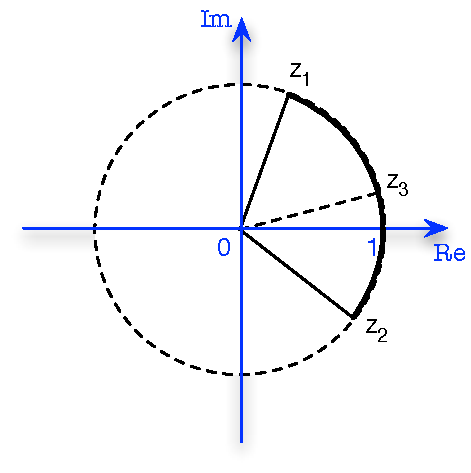
\includegraphics[width=88mm]{fig/ExampleArc_formal.pdf}
   \caption{计算单位复数$z_1,z_2$在复平面内角平分线$z_3$} \label{fig:midarc}
\end{figure*}

当$|z_1+z_2| < \epsilon$时,在程序代码的第4行与第5行,计算$z_1+z_2$时,由于$z_1 \approx -z_2$,这个加法操作会使得计算结果的有效数字位数发生锐减[],导致计算结果的相对误差非常大。而后续第7行的除法操作,由于除数$|z_1+z_2|$是一个非常小的数,会进一步放大前面加法操作的误差,导致程序的计算结果出错。我们实际运行了一下这个程序,在处理器为英特尔酷睿i7 2.9GHz的苹果笔记本MacBook Pro上,以浮点精度类型实现的该计算过程,我们令输入$z_1=e^{i\pi/4},z_2=-z_1*e^{-i \epsilon \pi},\epsilon=10^{-16}$,程序的运行结果$z_3=-0.5547+0.8321i$,显而易见是错误的,其正确结果应该为$z_3=-0.7071+0.7071i$。

\begin{figure}[thbp]
    \begin{lstlisting}[%
      xleftmargin=\columnsep,numberblanklines=true,boxpos=b,%,extendedchars=\true, %inputencoding=utf8%/latin1
      morekeywords={REAL,IComplex}%keywords={main}
    ]
    IComplex midarc(IComplex z1,IComplex z2){
      if(abs(z1)!=1 || abs(z2)!=1)
        throw PreConditionException;
      REAL r = realpart(z1) + realpart(z2);   
      REAL i = imaginary(z1) + imaginary(z2); 
      IComplex sum(r,i);
      IComplex z3 = sum / abs(sum);           
      return z3;
    }
    \end{lstlisting}
    %\vspace*{-4mm}
    \caption{直接使用公式$(z_1+z_2)/|z_1+z_2|$计算$z_3$的任意精度代码}
    \label{lst:exoricode}
    %\vspace*{-4mm}
\end{figure}
    
我们的优化框架可以将图\ref{lst:exoricode}中这样的不稳定的浮点精度的计算过程优化成为稳定高效的浮点精度的计算过程,如图\ref{lst:exoptcode}所示。 原来不稳定的计算过程$z_3=(z_1+z_2)/|z_1+z_2|$被转换成了一种与之在数学上等价的稳定的计算过程,具体来说,$z_1,z_2,z_3$均被表示成了复数的极坐标表示形式,$z_1=e^{i\theta_1},z_2=e^{i\theta_2}$,与此同时,$z_3$的计算过程也被等价的转换成为:

\begin{align}\label{eq:optex}
    z_3=e^{i\frac{\theta_1+\theta_2}{2}}
\end{align}

当$|z_1+z_2|<\epsilon$时,优化后的代码便使用这样稳定的计算过程来计算$z_3$,这样一来,优化后的代码便避免了原本不稳定的计算操作。同样的,我们以输入z$z_1=e^{i\pi/4},z_2=-z_1*e^{-i \epsilon \pi},\epsilon=10^{-16}$来运行优化后的代码,得到的结果即为正确的运行结果$z_3=-0.7071+0.7071i$。

\begin{figure}[thbp]
  \begin{lstlisting}[%
    xleftmargin=\columnsep,numberblanklines=true,boxpos=b,%,extendedchars=\true, %inputencoding=utf8%/latin1
    morekeywords={FComplex}%keywords={main}
  ]
  FComplex midarc(FComplex z1,FComplex z2){
    if((abs(z1)-1)>epsi || (abs(z2)-1)>epsi)
      throw PreConditionException;
    double r = realpart(z1) + realpart(z2);      
    double i = imaginary(z1) + imaginary(z2);    
    FComplex sum(r,i); FComplex z3;              
    if(abs(sum)<epsi){
      double theta1 = atan2(imaginary(z1),realpart(z1));
      double theta2 = atan2(imaginary(z2),realpart(z2));
      double theta3 = (theta1+theta2)/2;
      z3 = FComplex(cos(theta3),sin(theta3));
    }else{
      z3 = sum / abs(sum);                       
    }
    return z3;
  }
  \end{lstlisting}
  %\vspace*{-4mm}
  \caption{优化后的计算$z_3$的浮点精度代码}
  \label{lst:exoptcode}
  %\vspace*{-4mm}
\end{figure}

整个优化过程的主要思想是通过代数式的等价转化,将原本不稳定的浮点精度计算过程替换成为一个与之等价的稳定的计算过程,每次这样的计算过程的替换都必须保证替换前后的计算过程在数学意义上是等价的。这样的替换过程的主要难点在于如何自动地寻找这样一个等价的稳定计算过程,因此本文提出了一种基于随机代数变换的等价表达式搜索算法,将这样一个替换过程转变成为一个搜索的过程。首先,我们会将数值程序的计算过程作为一个整体抽取出来,得到一个计算过程的代数式(在上述例子中,这个代数式便是$z_3=(z_1+z_2)/|z_1+z_2|$),然后我们对该代数式进行随机的代数变换,变换过程以及得到的等价代数式集合如图\ref{fig:eqspace}所示,得到等价代数式集合后,我们会在整个等价集合中随机选取代数式然后继续进行随机的变换,这样迭代下去,一直到我们寻找到一个稳定的计算代数式。当我们找到了稳定的计算代数式后,我们会将这个代数式还原成为可执行代码,并替换原不稳定的计算过程。

\begin{figure}[thb]
  \centering
  \vspace*{1mm}
  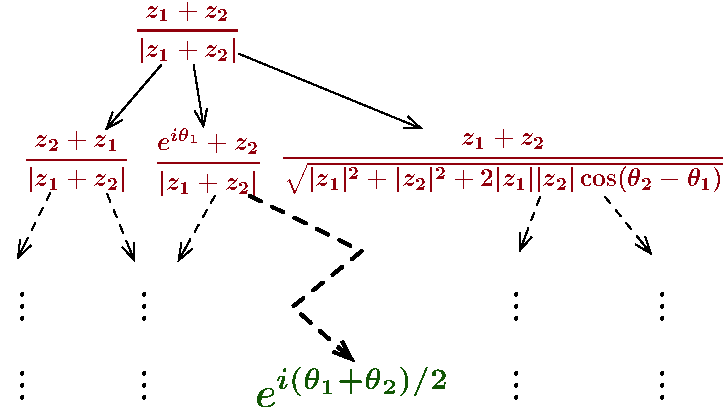
\includegraphics[width=120mm]{fig/EquivalentSpace.pdf}
  \vspace*{1mm}
  \caption{等价代数式变换过程及得到的等价代数式集合} \label{fig:eqspace} %Equivalence Space to Find a Stable Algebraic Form
\end{figure}

\section{方法框架}

在上一小节中我们以一个具体的实例说明了整体的优化过程,在这一小节中,我们将会具体讨论优化框架的具体构成以及一些技术细节。首先,数值程序的优化过程一共分为4个模块,如图\ref{fig:mainframe}所示,包括了稳定性分析模块、计算路径提取模块、随机代数变换模块以及计算路径合并模块。

首先,稳定性分析模块会使用区间分析的技术对原程序进行稳定性的分析,对程序的输入域进行划分,将程序的输入域划分为稳定区间,不稳定区间以及未知区间,这三种不同类型区间的具体含义会在下面具体介绍。紧接着,计算路径提取模块会通过符号执行的方式,将不稳定区间所对应的计算过程进行提取,得到程序输出关于程序输入的一个计算代数形式。然后,随机代数变换模块对上个模块提取到的计算代数式进行数学意义上的等价变换,寻找到原计算过程的等价的稳定的计算形式。最后,路径合并模块将上个模块中的等价稳定计算形式转换成为代码片段,并与原本就稳定的计算路径进行合并,得到最终的优化后程序。

\begin{figure*}[thbp]
  \centering
 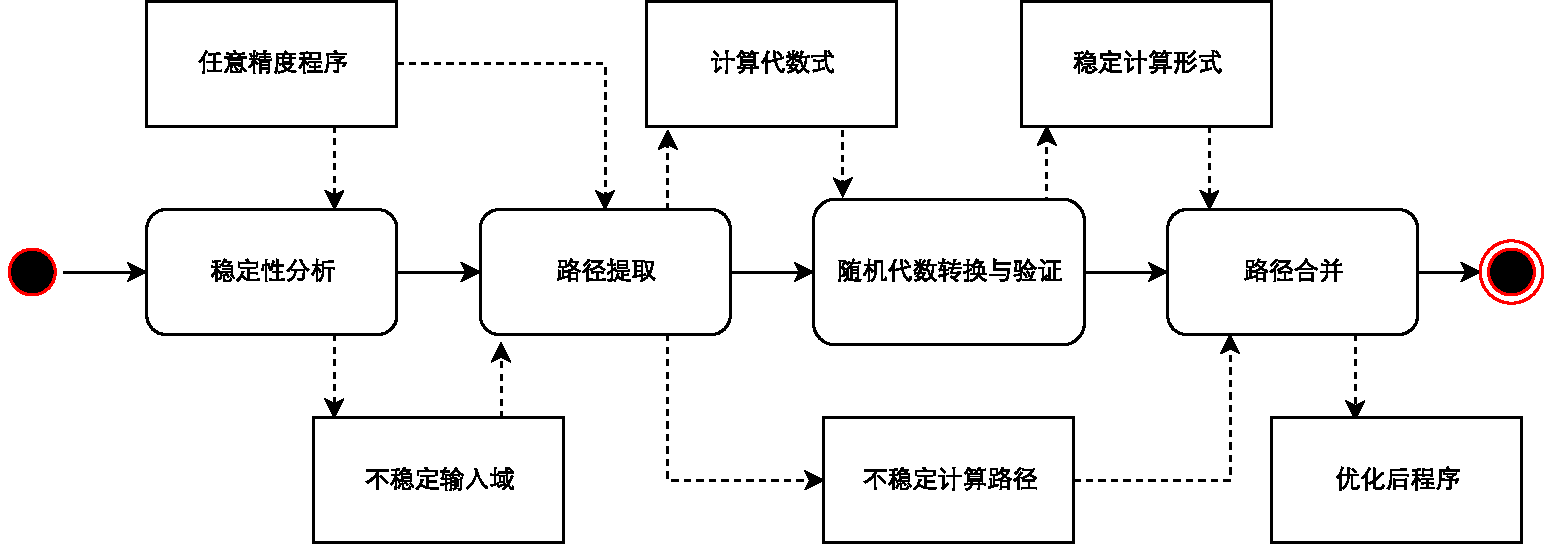
\includegraphics[width=\textwidth]{fig/MainFramework.pdf}
  \caption{数值程序优化框架整体流程图} \label{fig:mainframe}
\end{figure*}

\subsection{稳定性分析}

\subsubsection{稳定输入域定义}
对于一个计算过程$f$来说,我们记其浮点精度实现与任意精度实现所对应的计算过程分别为$F$和$M$,$D$为程序的输入域,对于任意输入$x \in D$,记$F(x)$与$M(x)$分别为以输入$x$去执行计算过程$f$的浮点精度实现以及任意精度实现所得到的计算结果。如果对一个输入域$I \subseteq D$,$I$上的任意输入$x$满足:

\begin{align}
  |\frac{F(x)-M(x)}{M(x)}| < \epsilon
\end{align}

则我们称该输入域$I$为一个稳定的输入域。反之,若存在$x \in $,使得:

\begin{align}
  |\frac{F(x)-M(x)}{M(x)}| \geq \epsilon
\end{align}

则我们称该输入域为不稳定输入域,其中$\epsilon$为参数,是一个很小的正数,用来表示优化框架所能容忍的最大的相对误差。

\subsubsection{输入域划分}

稳定性分析模块会将程序的输入域划分成为稳定输入域以及不稳定输入域,对于稳定输入域部分,由于其本身计算过程已经是稳定的,我们只需要将原计算过程直接使用浮点精度实现即可(对应图\ref{lst:exoptcode}中第13行),然而对于不稳定的输入域,其中包含了会产生误差的输入,优化框架需要对这样的输入域对应的计算过程进行优化(对应图\ref{lst:exoptcode}中第8行到第11行)。

如图\ref{fig:inputspace}为对数值计算程序输入域的一个整体的划分。理论上来讲,整个输入域可以完全的划分成为两个不相交的集合分别为稳定输入域以及不稳定输入域,然而这项工作在现实实践中是非常困难的。通过本节所介绍的分析技术,稳定性分析模块可以识别出部分的稳定输入域以及不稳定输入域,而剩余的无法识别的部分稳定性分析模块会将其归入未知输入域。在整个优化框架中,对于未知输入域以及无法找到稳定计算过程的不稳定输入域,我们会保留原始的任意精度计算过程以保证程序最终计算结果的正确性。

\begin{figure}[tb]
  \centering
  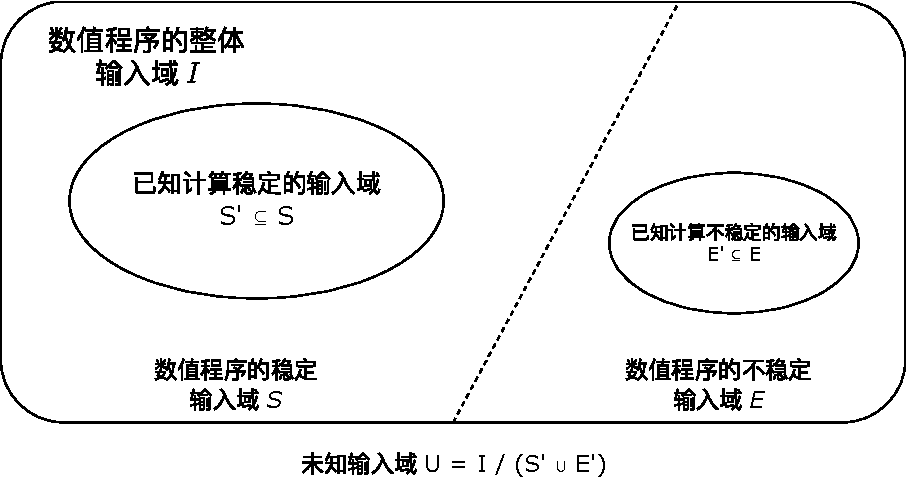
\includegraphics[width=\columnwidth]{fig/InputSpace.pdf}
  \vspace*{1mm}
  \caption{数值计算程序输入域划分图} \label{fig:inputspace} %Equivalence Space to Find a Stable Algebraic Form
\end{figure}

\subsubsection{稳定性分析方法}

稳定分析的整体算法流程如算法\ref{alg:stabilityAnalysis}所示,首先我们会将程序的输入域划分为许多小区间,然后我们对每个小区间的稳定性进行判定,然后再将相同类型的小区间组合起来得到最终的稳定输入域,不稳定输入域以及未知输入域。对于每个小区间,首先,我们会使用区间分析的技术判定该小区间上的最大误差是否在一个可接受的范围内,如果是,我们则认为该小区间是稳定的,将其加入到稳定输入域中。紧接着,如果我们无法判定小区间是稳定的,我们会尝试着去在其中寻找不稳定的输入,我们会在该小区间上随机取一些输入点,将这些输入带入原始任意精度计算过程以及对应的浮点精度计算过程,得到两种计算过程结果的相对误差,若发现有产生较大误差的输入,我们则判定该小区间是不稳定的,否则我们将其纳入未知输入域,因为我们既无法证明该区间是稳定的,又无法找到该区间中的不稳定输入。

\begin{algorithm}[thb]
  \caption{Stablility Analysis Process}
  \label{alg:stabilityAnalysis}
\begin{algorithmic}[1]
\REQUIRE $D$ {{\footnotesize$//$}\small Input Space}
\ENSURE $S', E', U$ {{\footnotesize$//$}\small Stable subspace, Unstable subspace and Unknown subspace}
\STATE $S_d$ $\leftarrow$ split($D$) {{\footnotesize$//$}\small Split input space to a set of small intervals}
\FORALL {$d \in D$}
\IF {$isIntervalStable(d)$}
\STATE add($d$, $S'$)
\ELSE
\STATE $S_p$ $\leftarrow$ randomSamplePoints($d$) {{\footnotesize$//$}\small Randomly sample a few points in $d$}
\FORALL {$p \in S_p$}
\IF{$\neg$ checkStable($p$)}
\STATE add($d$, $E'$)
\ENDIF
\ENDFOR
\STATE add($d$,$U$) {{\footnotesize$//$}\small All sampled points are stable, can't tell whether stable or not}
\ENDIF
\ENDFOR
\end{algorithmic}
\end{algorithm}

\subsection{路径提取}
为了对不稳定输入域上的计算过程进行优化,我们必须将这些计算过程作为一个整体从程序中提取出来,整个计算过程被抽象成为了程序输出关于程序输入的一个计算代数式的形式,这便是路径提取模块所要完成的工作。并且,对于不同输入域上的输入,其对应的计算过程有可能是不同的,对应到程序的控制流图上,即程序在不同输入域上在程序控制流图上所执行的路径时不同的,我们需要对不稳定输入域上涉及到的所有的程序执行路径进行提取。在对程序的执行路径进行提取的同时,路径提取模块同时还会收集每一条执行路径所对应的约束,以便于后续计算过程优化结束后组合程序时使用。原计算过程经过路径提取后被抽象成为了$\{(Constrain, AlgebraForm)\}$这样的二元组的集合的形式,集合中每个元素均为一个二元组,代表了程序控制流图中的一条执行路径,包含了该执行路径的计算代数式以及对应的约束信息。

下面举一个具体的实例来描述路径提取模块的执行结果,如图\ref{lst:symextexam}所示为计算$f(a,b)=|a|+|b|$的数值程序代码片段。显而易见,此程序中总共包括了4条不同的执行路径,优化框架对其进行路径提取的结果如表\ref{tbl:abssumres}所示,不同约束下对应了不同的计算过程。

\begin{figure}[thbp]
    \begin{lstlisting}[%
      numberblanklines=true,boxpos=b,%,extendedchars=\true, %inputencoding=utf8%/latin1
      morekeywords={REAL,IComplex}%keywords={main},
      xleftmargin=.2\textwidth, xrightmargin=.2\textwidth
    ]
    double abs_sum(double a, double b) {
      double r = 0.0;
      if ( a > 0 ) { r += a; } 
      else { r -= a;}
      if ( b > 0 ) { r += b; }
      else {r -= b;}
      return r;
    }
    \end{lstlisting}
    %\vspace*{-4mm}
    \caption{计算$f(a,b)=|a|+|b|$代码片段}
    \label{lst:symextexam}
    %\vspace*{-4mm}
\end{figure}

\begin{table}
  \centering
  \begin{tabular}{ccc}
    \toprule
    \textbf{路径编号} & \textbf{路径约束} & \textbf{计算代数式} \\
    \midrule
    1 & a>0\&\&b>0 & a+b \\
    2 & !(a>0)\&\&b>0 & -a+b \\
    3 & a>0\&\&!(b>0) & a+(-b) \\
    4 & !(a>0)\&\&!(b>0) & (-a)+(-b) \\
    \bottomrule
  \end{tabular}
  \caption{数值计算程序$f(a,b)=|a|+|b|$路径提取结果}\label{tbl:abssumres}
\end{table}

路径提取模块主要使用的符号执行这一技术来完成对计算路径的提取。符号执行是一种广泛用于程序分析、软件安全和软件测试的技术,符号执行于20世纪70年代被提出,至今已经取得了长足的发展。不同于具体的执行,符号执行使用符号化的变量代替程序具体的输入,一步步地执行程序,在执行过程中,所有的中间变量也以符号表达式的形式记录下来。当遇到分支语句时,符号执行会产生新的状态以记录不同的执行分支。

原始的符号执行技术主要用于测试用例生成,当符号执行结束后得到了不同执行路径的约束后,通过将约束交给约束求解器求解可以得到覆盖该执行路径的测试用例。在我们的框架中我们对原始的符号执行技术进行了改进,使其不仅仅记录路径约束,同时也会记录每条执行路径所对应的执行结果。在符号执行过程中,对于程序中每一条执行路径,我们会维护一个符号执行的状态信息$es=(ins, sym, out, c)$,其中$es.ins$表示当前被执行指令,$es.sym$记录了到现在为止的符号执行过程中所收集到的变量以及其对应的符号表达式,$es.out$记录了数值计算程序的所有的输出的变量,最后$es.c$表示执行路劲对应的约束信息。当一个程序执行状态遇到了一条分支指令时,该执行状态也会对应地产生两个新的执行状态$es_1$与$es_2$,分别对应了分支指令的$True$分支与$False$分支。若分支条件为$b$,则$es_1$的路径约束被更新成为$es.c \wedge b$,对应的$es_2$的分支条件则为$es.c \wedge \neg b$。

\begin{algorithm}[thb]
  \caption{Symbolic Trace Extraction Process}
  \label{alg:tractExtract}
\begin{algorithmic}[1]
\REQUIRE $\mathcal{P}, S'$ \hfill {{\footnotesize$//$}\small input program \& stable subspace}
\ENSURE $M_{AF}$ \hfill {{\footnotesize$//$}\small map every output to an algebraic form} %[e_1,\cdots,e_n]
    \STATE $es$ $\leftarrow$ initialSTATE($\mathcal{P}$);
    \FORALL {$i \in$ input($\mathcal{P}$) $\wedge\ i \in \mathbb{F}$}
      \STATE add($es.sym$, $i$); \hfill {{\footnotesize$//$}\small\ declare inputs to be symbols} \label{alg:tractExtract:input}
    \ENDFOR
    \STATE $ES$ $\leftarrow$ \{$es$\}; \hfill {{\footnotesize$//$}\small $ES$ is a state set}
    \WHILE{$\neg$empty($ES$)} \label{alg:tractExtract:iter}
      \STATE $es \leftarrow$ selectSTATE(ES); \label{alg:tractExtract:select}  \hfill {{\footnotesize$//$}\small $es$ is the current state}
      \SWITCH{$es$.$ins$.Type}
      \CASE {fork \hfill {{\footnotesize$//$}\small such as the \texttt{if} statement} \label{alg:tractExtract:fork}}
        \STATE \{$es_1,es_2$\}$\leftarrow$ forkExecution($es$);
        \STATE \textbf{if} {$\exists i \notin S'$, $es_1.c$($i$)} \textbf{then} add(ES, $es_1$);
        \STATE \textbf{if} {$\exists i \notin S'$, $es_2.c$($i$)} \textbf{then} add(ES, $es_2$);
        \STATE remove(ES, $es$);   \label{alg:tractExtract:forkend}
      \ENDCASE
      \CASE {OUTPUT($v$) $\wedge\ v \in \mathbb{F}$ \hfill {{\footnotesize$//$}\small such as \texttt{printf}($v$)}}
        \STATE add($es.out$, $v$); \label{alg:tractExtract:outputv}
      \ENDCASE
      \CASE{$\mathcal{P}$.EXIT} %\hfill {\small$\triangleright$such as \texttt{abort}, \texttt{exit}} \label{alg:main:exit_statement}
        \FORALL {$v \in es.out$}
          \STATE add($M_{AF}$, symtraceAF($v$, $es$)); \label{alg:tractExtract:recordexp} % 我这里没有写, 事实上这一步非常复杂. symtraceAF 会返回一个对应关系 <v, af<v>>, 同时会记录es.c, 真正记录到$M_{AF}$中的是<v, es.c, af<v>>, 如果另一个路径也输出v, 会有不同的es.c
        \ENDFOR
        %\STATE Generate Algebric Forms for V;  \label{alg:tractExtract:v}
        \STATE remove(ES, $es$);
      \ENDCASE
      \DEFAULT
        \STATE symbolicStep($es$); \label{alg:tractExtract:propagationstep}
      \ENDDEFAULT
      \ENDSWITCH  \label{alg:tractExtract:switend}
    \ENDWHILE \label{alg:tractExtract:iterend}
\end{algorithmic}
\end{algorithm}

算法\ref{alg:tractExtract}描述了此模块中使用到的符号执行技术的具体算法流程,首先我们会将所有的输入变量符号化,然后我们便一步步的以符号执行的方式执行程序。当遇到一条分支语句时,便产生不同的不同的执行状态以记录不同的执行分支(第9行至第13行),同时我们的符号执行过程也会收集程序输出所对应的计算表达式(第14、15行),当程序结束时,将所有记录到的程序输出的计算表达式添加到结果集中去(第16行至第20行),剩余的情况则按照正常的符号执行过程来执行。

\subsubsection{循环模型与递归模型}
% TODO

\subsection{随机代数变换}

\subsection{路径合并}

